This chapter outlines the methodological approach adopted to measure liquidity risk and investors' sentiment, along with their rationale. These factors are integrated into an enhanced asset pricing framework based on the FF5 and C4F. Subsequently, the implementation of the Random Forest (RF) algorithm is detailed. Next, the rule-based model will be extracted from the RF for comparison and application to the Association Rule Learning Sector Rotation Strategy.



\subsection{Liquidity Risk factor}
The construction of liquidity factors closely aligns with the methodology outlined by \citeA{gu_2020}. The authors include a comprehensive suite of seven stock-level liquidity proxies: turnover and turnover volatility (\texttt{turn}, \texttt{SDturn}), log market equity (\texttt{mvel1}), dollar volume (\texttt{dolvol}), Amihud illiquidity (\texttt{ILLQ}), number of zero trading days (\texttt{zerotrade}), and bid-ask spread (\texttt{baspread})—to capture the multifaceted nature of trading costs and depth. Turnover measures trading frequency (\[\frac{Number of shares traded}{Number of outstanding shares}\]), while its standard deviation (\texttt{SDturn}) captures episodic illiquidity shocks (stocks with infrequent or highly variable trading demand higher expected returns as compensation). Log market equity (\texttt{mvel1}) and dollar volume (\texttt{dolvol}) proxy for firm size and the how active the market is, respectively, since smaller firms and low-\texttt{dolvol} issues exhibit thinner order-book depth (not a lot of people are buying and selling). Bid-ask spread (\texttt{baspread}) directly reflects immediacy costs, and a wider spread signals greater liquidity risk. The count of zero-trading days (\texttt{zerotrade}) quantifies outright market “gaps” where trading is impossible (your equity literally cannot be liquidated), each gap intensifying illiquidity premia. Finally, Amihud's \texttt{ILLQ}—defined as
\begin{equation}
\label{eq:amihud}
\text{ILLIQ}{i,y} ;=;\frac{1}{D_i^y}\sum{d=1}^{D_i^y}\frac{|R_{i,d}|}{VOL_{i,d}}
\end{equation}
where $R_{i,d}$ is the daily return and $VOL_{i,d}$ the dollar trading volume for stock $i$ on day $d$, scaled by $10^6$ to ease interpretation—captures the price impact per dollar traded \citeA{amihud_2002}. By including proxies for trading frequency, volume scale, price impact, cost of immediacy, and market “holes,” \citeA{gu_2020} ensure that no single dimension of illiquidity is overlooked, and empirical tests confirm that different measures emerge as top predictors of future returns in varying market environments.



\subsection{Sentiment}
%% OUTLINE: wurgler -> antoniu -> XU enhanced
\citeA{wurgler_2006} constructed a sentiment index (BW index hereafter) by capturing the principal components within six proxies: closed-end fund discount (\texttt{CEFD}), NYSE share turnover (\texttt{turn}), the number and average first-day returns of IPOs (\texttt{NIPO, RIPO} respectively), equity share in new issues (\texttt{S}) and dividend premium (\texttt{P}). \footnote{However, by March 2016, the NYSE share turnover proxy has been dropped in the database due to "the explosion of institutional high-frequency trading and the migration of trading to a variety of venues" \cite{ung_2023}}%can definitely add more after the proposal here, from the paper

The sentiment is calculated as follows:
\begin{equation}
    \label{eq:sentiment}
    \begin{split}
    \text{SENTIMENT}_t = -0.241\,\text{CEFD}_t + 0.242\,\text{TURN}_{t-1} \\ + 0.253\,\text{NIPO}_t 
    + 0.257\,\text{RIPO}_{t-1} \\ + 0.112\,S_t - 0.283\,P^{D-ND}_{t-1} , 
    \end{split}
\end{equation}

where each proxy has been standardized. $\text{D}-\text{ND}$ is the difference between dividend payers and non-dividend payers. Principal Component Analysis(PCA) reveals the hidden common factor from this group of factors by transforming the data into principal components (PCs) that would capture as much variance in the data as possible. PC1 should capture the maximum variation from the sentiment proxies, thereby serving as an aggregate measure of investor sentiment. Since both market sentiment and the business cycle can drive common variation in financial data, the PCA will treat both as sources of variance without distinguishing whether that variance comes from changes in investor sentiment or broader macroeconomic factors. A second orthogonalized index is formed by regressing each of the proxy with independent variables that explains the business cycle. The residuals of this regression will be the 'pure" sentiment, which is the variation that the macroeconomic factors fail to explain. The following is the orthogonalized index, with $\perp$ labelling the removal of business cycle. 

\begin{equation} %BEQ
    \label{eq:sentiment_orth}
    \begin{split}
    \text{SENTIMENT}^{\perp}_t = &-0.198\,\text{CEFD}^{\perp}_t + 0.225\,\text{TURN}^{\perp}_{t-1} \\
    &+ 0.234\,\text{NIPO}^{\perp}_t + 0.263\,\text{RIPO}^{\perp}_{t-1} \\
    &+ 0.211\,S^{\perp}_t - 0.243\,\text{P}^{\text{D} - \text{ND},\perp}_{t-1}
    \end{split}
\end{equation}

However, \citeA{ung_2023} pointed out several problems with the BW index. First, though it has robust predictive perfomance on a cross- sectional level, it is weak for aggregate market retuerns in time series regressions - even \citeA{wurgler_2007} pointed this out themselves in the paper. Second, the BW index assumes that the contributions of each sentiment proxy to the aggregate index are fixed over time. Finally, the index has `look ahead bias': PCA uses the whole sample, and forecasts at time $t$ should not rely on data that would only become available after $t$. Therefore, \citeA{ung_2023} constructed an enhanced index to address these problems. The time-varying BW sentiment index ($S^{TV}$ hereafter) is constructed on a three years rolling window basis to use the most up-to-date information at each $t$, and is built upon \cref{eq:sentiment_orth}. This rolling window allows the model to adjust to structural breaks in the market without distorting the sentiment index. Furthermore, adjustments to the sign of the RICO proxy display a negative initial loading. This paper will use \citeA{ung_2023} $S^{TV}$ index to measure investors' sentiment.

In addition to the Enhanced BW index, the Daily News Sentiment Index from the Federal Reserve Bank of San Francisco provides a high-frequency gauge of U.S. economic sentiment, capturing short-run fluctuations in public perceptions as reported by major national newspapers. Specifically, the index aggregates sentiment scores derived from economics-related articles in 24 leading U.S. newspapers, including those with nationwide reach such as the \emph{New York Times} and the \emph{Washington Post}. Articles included in the measure must contain at least 200 words and be classified by Factiva (a news aggregator) as pertaining to "economics" and the "United States". To generate the sentiment score, \citeA{shapiro_2020} combine general-purpose sentiment dictionaries with a custom, news-specific lexicon to more accurately reflect the tone and context of economic reporting. Sentiment is scored at the article level and then aggregated using a trailing weighted average, in which more recent articles receive higher weights, with geometric decay over time. This method makes sure that any adjustments for potential shifts in the composition of the newspapers within the index is accounted for.

Complementing the two official sentiment indexes, this paper also utilizes a proxy for sentimet, the Volatility Index (VIX hereafter). The VIX, commonly reffered to in the finance sector as the 'fear index' computes a 30 day forward-looking estimate of market volatility by aggregating the prices of out-of-the-money S\&P 500 index options, weighted across a broad range of strike prices and interpolated to produce a constant maturity of 30 days. It uses both put and call options with expirations between 23 and 37 days, along with current U.S. Treasury rates, to accurately reflect current market expectations. The formula essentially replicates a theoretical variance swap—summing the contributions from each eligible option—then takes the square root and annualizes the result (WHAT IS THE FORMULA). 

(EXPLAIN WHAT BETA AND ALPHA IS)


\subsection{Factor models}
%%%%%%ACTUAL%%%%%%
This thesis will employ two CAPM variants: the C4F of \citeA{cahart_1997} and FF5 of \citeA{ff5_2015}. The following are their respective formulas:

\begin{equation}
    \label{eq:c4f}
    \begin{split}
        R_{i,t} - R_{f,t} &= \alpha_i + \beta_{MKT} (R_{MKT,t} - R_{f,t}) \\
        &\quad + \beta_{SMB} \cdot SMB_t + \beta_{HML} \cdot HML_t \\
        &\quad + \beta_{MOM} \cdot MOM_t + \epsilon_{i,t}
    \end{split}
\end{equation}

\begin{equation}
    \label{eq:ff5}
    \begin{split}
        R_{i,t} - R_{f,t} &= \alpha_i + \beta_{MKT} (R_{MKT,t} - R_{f,t}) \\
        &\quad + \beta_{SMB} \cdot SMB_t + \beta_{HML} \cdot HML_t \\
        &\quad + \beta_{RMW} \cdot RMW_t + \beta_{CMA} \cdot CMA_t + \epsilon_{i,t}
    \end{split}
\end{equation}

where \cref{eq:c4f} is the C4F and \cref{eq:ff5} is the FF5. $R_{i,t}$ is the return on security and $R_{f,t}$ is the risk-free return; which makes $R_{i,t} - R_{f,t}$ is the excess return on a security. $SMB$ (small minus big) is the size factor, capturing the excess returns of small-cap stocks over large-cap stocks, reflecting how higher volatility and growth potential could cause smaller firms to yield higher average returns. $HML$ (high minus low), or the value factor, accounts for the premium earned by stocks with high book-to-market ratios, often associated with underperforming firms that carry higher risk and, consequently, higher expected returns \cite{ff3_1993}. $MOM$ is the one year momentum factor \footnote{In literature, researchers can refer to this factor as PR1YR, UMD (ups minus downs), or WML (winners minus losers.)} \cite{cahart_1997}. In response to \citeA{titman_2004} and \citeA{novymarx_2013} criticisms, two additional factors were added in to the FF3 model \cite{ff5_2015}. $RMW$ (robust minus weak) is the profitability factor, which derives from the empirical observation that firms with higher operating profitability tend to earn higher average returns. $CMA$ (conservative minus aggressive) is the investment factor, which captures the tendency of firms to aggressively invest in new assets, expecting higher returns in the long run. Investors may overpay for such firms due to optimism, which results in lower subsequent returns \cite{titman_2004}.

The empirical analysis will begin by establishing a baseline for each asset pricing variant using time series regressions, employing Ordinary Least Squares (OLS) as outlined by \citeA{simonian_2019}. \cref{eq:c4f} and \cref{eq:ff5}, the two baseline variants will be referred to as C4F-B and FF5-B hereafter. Subsequently, liquidity risk and sentiment indicators will be integrated into these variants, thereby forming an enhanced baseline. The following are the enhanced baseline models:

\begin{equation}
    \label{eq:c4f_expanded}
    \begin{split}
    R_{i,t} - R_{f,t} &= \alpha_i + \beta_{MKT} (R_{MKT,t} - R_{f,t}) \\
    &\quad + \beta_{SMB} \cdot SMB_t + \beta_{HML} \cdot HML_t \\
    &\quad + \beta_{MOM} \cdot MOM_t \\
    &\quad + \beta_{turn} \cdot TURN_{i,t} + \beta_{SDturn} \cdot SDTURN_{i,t} \\
    &\quad + \beta_{mvel1} \cdot MVEL1_{i,t} + \beta_{DOLVOL} \cdot DOLVOL{i,t} \\
    &\quad + \beta_{ILLQ} \cdot ILLQ_{i,t} + \beta{zerotrade} \cdot ZEROTRADE_{i,t} \\
    &\quad + \beta_{baspread} \cdot BASPREAD_{i,t} + \epsilon{i,t}
    \end{split}
\end{equation}

\begin{equation}
    \label{eq:ff5_expanded}
    \begin{split}
    R_{i,t} - R_{f,t} &= \alpha_i + \beta_{MKT} (R_{MKT,t} - R_{f,t}) \\
    &\quad + \beta_{SMB} \cdot SMB_t + \beta_{HML} \cdot HML_t \\
    &\quad + \beta_{RMW} \cdot RMW_t + \beta_{CMA} \cdot CMA_t\\
    &\quad + \beta_{turn} \cdot TURN_{i,t} + \beta_{SDturn} \cdot SDTURN_{i,t} \\
    &\quad + \beta_{mvel1} \cdot MVEL1_{i,t} + \beta_{DOLVOL} \cdot DOLVOL{i,t} \\
    &\quad + \beta_{ILLQ} \cdot ILLQ_{i,t} + \beta{zerotrade} \cdot ZEROTRADE_{i,t} \\
    &\quad + \beta_{baspread} \cdot BASPREAD_{i,t} + \epsilon{i,t}
    \end{split}
\end{equation}

where \cref{eq:c4f_expanded} is the enhanced C4F baseline (C4F-BE) and \cref{eq:ff5_expanded} the enhanced FF5 enhanced baseline (FF5-BE). 


\subsection{Random Forest}

%%%%%%%%OUTLINE%%%%%%%%%%
%Factor models are generally linear. Which kinds of regression are they usally used with (fama macbeth)? 


%%%%%%%%%%ACTUAL%%%%%%%%%%%%%%%
The C4F-B, C4F-BE, FF5-B and FF5-BE, since based on OLS, are linear in nature. These models are favored by finance practitioners because they produce interpretable results. The main results that the practitioners look for is the sensitivities of the factor within the models, or the beta coefficients within the OLS. However, the method is constraint to several assumptions. The features and the target variables of this method are assummed to be linear and the features themselves are not multicollinear. Furthermore, homoskedactiy is assumed, where the residuals have constant variance at every level of the features. The residuals should also be independent.

%maybe motivate more why tree based methods.
ML models offer a more robust framework, especially decision tree based models such as Random Forest (RF). With regression based problems like asset pricing, decision trees start from a root node and splits into brances. Each branch contains a condition to be fullfilled (for example $turn > 10$ or $turn < 10$). A tree can have numerous amounts of these brances, leading to a complex model that can take into account non-linearity and interactions. The leaf of the decision tree, or the final prediction, is a real number that is predicted given all of the previous conditions in the branches are true \cite{cutler_2012}. This method ressembles multiple nested if-then statements, where each if-then statement is a branch of the tree. An example of a decision tree can be observed in Figure \cref{fig:decision_tree_viz}.

\begin{figure}[H]
    \centering
    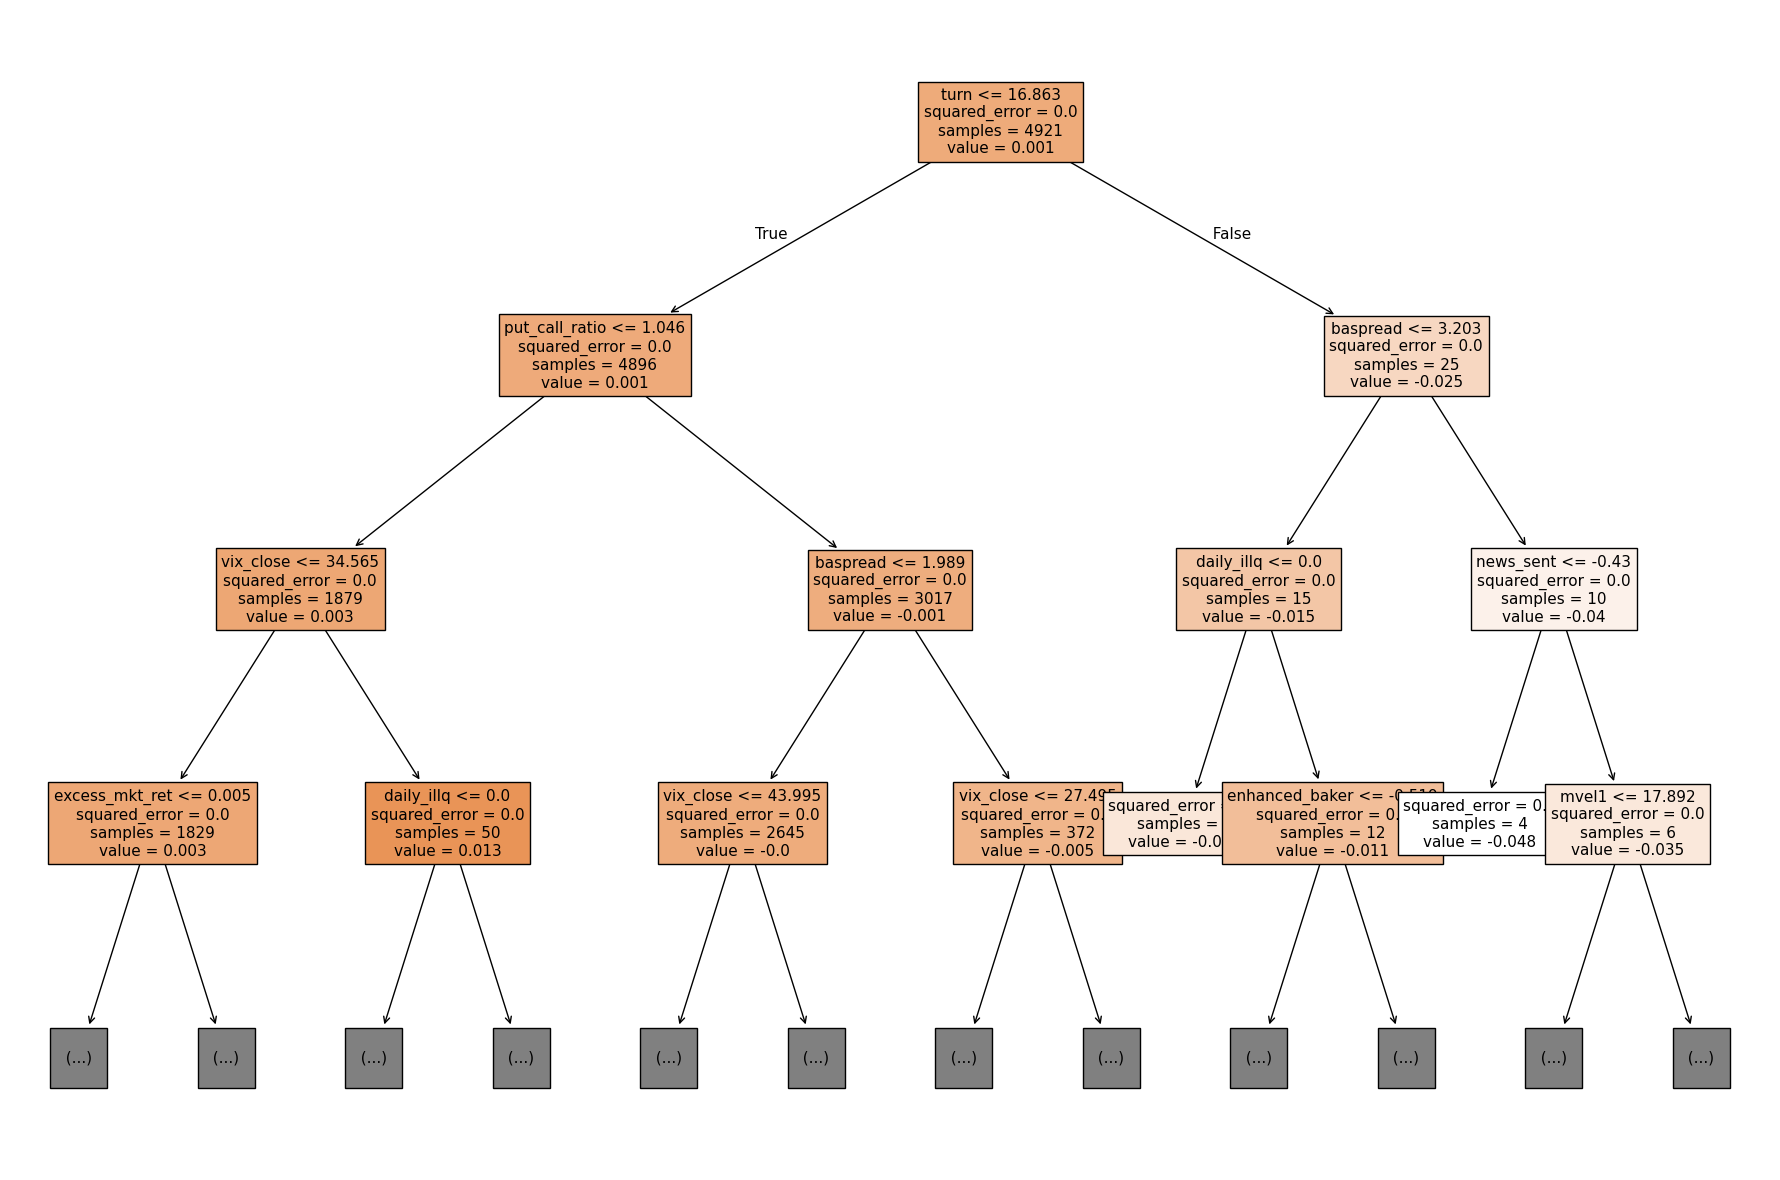
\includegraphics[width=\textwidth]{/Users/minhquangngo/Documents/vsc/erasmus/msc_thesis/latex/plots/methods/tree_example_one.png}
    \caption{Example of a decision tree.}
    \label{fig:decision_tree_viz}
\end{figure}

At its core, a regression tree tries to approximate an unknown regression function
\begin{equation}
    \label{eq:regression_tree}
    f(\mathbf{x})
    =
    \mathbb{E}[Y \mid \mathbf{X}=\mathbf{x}]
\end{equation}
by partitioning the $p$-dimensional predictor space into a set of disjoint rectangles (terminal nodes) and assigning a constant prediction (usually the sample mean of $Y$) to every rectangle.  The Classification-And-Regression-Tree (CART) algorithm (outlined in Algorithm \ref{alg:binary_recursive_partitioning}) achieves this with a binary recursive partition procedure that is entirely data-driven. Features are essentially evaluated based on how well they minimize the cost function, and the value that does it best is chosen as the split value. The Recursive Partitioning takes place at each layer of the tree and the value that is observed at each leaf is the mean of all observations in that node. % ASK GPT TO SEE IF THERE IS ANYTHIG WONG

\begin{algorithm}[H]
    \caption{Binary Recursive Partitioning}
    \label{alg:binary_recursive_partitioning}
    
    Let $\mathcal{D} = \{(x_1, y_1), \ldots, (x_n, y_n)\}$ denote the training data, with $x_i = (x_{i,1}, \ldots, x_{i,p})^T$.
    
    \Begin{
        Start with all observations $(x_1, y_1), \ldots, (x_n, y_n)$ in a single node.\;
        
        Repeat the following steps recursively for each unsplit node until the stopping criterion is met:\;
        \Indp
        \Begin{
            Find the best binary split among all binary splits on all $p$ predictors.\;
            Split the node into two descendant nodes using the best split (step 2a).\;
        }
        \Indm
        
        For prediction at $x$, pass $x$ down the tree until it lands in a terminal node. Let $k$ denote the terminal node, and let $y_{k_1}, \ldots, y_{k_n}$ denote the response values of the training data in node $k$. Predicted values of the response variable for regression are given by $\hat{h}(x) = \bar{y}_k = \frac{1}{n} \sum_{i=1}^n y_{k_i}$\;
        Source: \cite{cutler_2012}
    }
    \end{algorithm}

(THEN RF IS A COLLECTION OF DECISION  TREES...)


Non-linear relationships can be captured and multicollinearity could be dealt with. Furthermore, unlike OLS, RF models are estimated without the inversion of the covariance matrix. Parametric assumptions are not required, therefore heteroskedacity and non-independence of errors are accepted. The following RF implementation follows \citeA{simonian_2019}. In the RF model, each factor in \cref{eq:c4f,eq:c4f_expanded,eq:ff5,eq:ff5_expanded} can be represented as a feature to predict the excess return of the security. The baseline equivalent for the RF are named, respectively C4F-RF, C4F-RFE, FF5-RF, FF5-RFE. Stock returns forecasts are then aggregated by sector, which will then be divided into 10th, 25th, 50th, 75th, and 90th percentile. According to \citeA{simonian_2019}, this divide often show assymetric relationships within a set of observations. For example, certain features are more prevalent with low return portfolios than high return portfolios.

A downside of RF (and most other ML models) is their "black-box" nature, where their inner workings are unintuitive, which makes it unattractive to many investment professionals. RF captures non-geometric relationships between factors, therefore it is not analogous to the interpretation of common methods in the financial field (OLS, PCA). However, there are still multiple ways that can give investors insights into the RF black-box. The most common method utilized is the Relative Feature Importance (RFI hereafter), which weighs all of the factors within the RF according to their predictive robustness. \citeA{simonian_2019} attemted to generate what is similar to "betas" in traditional asset pricing models from RFI. An accepted understanding of "betas" in linear models is the elasticity of one variable to another, therefore a RFI-weighted elasticity, or "psuedo-beta" is constructed:
%EXPLAIN MORE WHAT BETA ALPHA IS
\begin{equation}
    \label{eq:psuedo}
    \frac{\text{Target Variable value}}{\text{{Feature value}}}* \text{RFI}
\end{equation}

By utilizing this method, the interpretation of the RF models could be communicated with investment professionals who are more familiar with OLS betas or PCA loadings.


    
    

\subsection{Rule-based models}
There are statistical methods that only sacrifice a small amount of accuracy, but its inner workings are translated into "if-then" statements that could be communicated to investment managers. Rule-based models turns the “black box” RF into a transparent collection of "if-then" statements \cite{benard_2021}. Each rule summarizes a path of decisions about factor values. In this particular context, a rule could be “If $\texttt{ILLQ}$ exceeds a certain threshold and \texttt{HML} remains below a specific level, then $\texttt{Expected Excess Return} = x$.”. Such structures mirror how a practitioner might articulate investment strategies.

This intepretable rule based model is outlined in \citeA{benard_2021}, which introduces \textbf{S}table and \textbf{I}nterpretable \textbf{RU}le \textbf{S}et (SIRUS) for regression, based on RF. After the Random Forest is built, every possible condition-based rule that can come out of the trees is examined. Because each tree splits the data in different ways, some rules will appear in multiple trees, whereas others might appear only once. Rules that show up more frequently across the entire forest are considered more reliable because their conditions hold under various random draws and data subsets. Next, we choose a cutoff point to decide when a rule appears “often enough” to be considered important. If a rule meets or exceeds this cutoff in how frequently it shows up in the RF, we keep it; if not, we discard it. After keeping only the important rules, we bring them together into a single model. Essentially, each rule can give a “low” or “high” prediction, depending on whether its condition applies or not. We then assign a weight to each rule, so that the final prediction is just the sum of these weighted rules plus an overall baseline value. Because we only keep a handful of the most frequent rules, the end result is both more concise and easier to understand, resembling a clear list of if-then statements with associated weights. The best performing RF model out of C4F-RF, C4F-RFE, FF5-RF and FF5-RFE in predicting returns will be eligible for SIRUS rule extraction. This model will be referred to as RF-SIRUS hereafter.
 

\subsection{Sector rotation strategy}
The best RF variant and its SIRUS extraction will be adapted to a practical trading application, providing investors and practitioners in the field a tool that provide insights and guide them on investment decisions. After the RF and SIRUS forecasts, the excess returns of each sector will be aggregated by sector for the month ahead. With a sector rotation strategy, the sector that is held in the portfolio is the one that signals outperformance on the market. The sector rotation strategy implemented in this paper closely follows \citeA{simonian_2019} methods, using Association Rule Learning (ARL). The signals utilized by the authors are the one month ahead predicted returns and ratio of shorter-term to longer-term realized volatility (24-month vs. 36-month), which is calculated as follows:

\begin{equation}
    \label{eq:vol_ratio}
    VR_t = \text{Volatility ratio at time } t = \frac{\text{Volatility}(t-24, t)}{\text{Volatility}(t-36, t)}
\end{equation}
    

Generally, ARL searches through large observations to find association rules. It is a rolling-window learning approach, meaning it updates on new data that comes in. Instead of using a fixed model trained once on historical data, it re-estimates the relationships every 18 months, which is called a "look-back" window.  The idea is to discover whether certain thresholds of “predicted return” and “volatility ratio” tend to coincide with above-average returns in the following month. The sector will be owned in the portfolio if the following conditions are sastisfied \footnote{A more formal description will be provided in the Methods section of the thesis}:

\begin{equation}
    \label{eq:arl}
    (\text{Volatility ratio} < 1) \land (\text{RF-predicted return} > \alpha) \implies (\text{Sector return} > \beta)
\end{equation}

\subsection{S\&P500 as a benchmark}


%iterative add factor de xem la feature importance co doi ko 